\documentclass{article}
\usepackage{pdfpages}
\usepackage{listings}
\usepackage[T1]{fontenc}
\usepackage{xcolor}
\usepackage{placeins}
\usepackage{float}
\usepackage{underscore}
\usepackage[bookmarks=true]{hyperref}
\usepackage[utf8]{inputenc}
\usepackage[margin=0.5in]{geometry}
\usepackage{graphicx}
\usepackage{subfigure}
\usepackage[english]{babel}
\hypersetup{
	bookmarks=false,    % show bookmarks bar?
	pdftitle={Text Analytics Tutorial 3},    % title
	pdfauthor={Adam-Ryan},                     % author
	pdfsubject={TeX and LaTeX},                        % subject of the document
	pdfkeywords={TeX, LaTeX, graphics, images}, % list of keywords
	colorlinks=true,       % false: boxed links; true: colored links
	linkcolor=blue,       % color of internal links
	citecolor=black,       % color of links to bibliography
	filecolor=black,        % color of file links
	urlcolor=blue,        % color of external links
	linktoc=page            % only page is linked
}%
\def\myversion{1 }
\date{}
%\title
\usepackage{hyperref}
\begin{document}
	
\section{Exercise 1}
This is the answer to question 1.
\begin{enumerate}
	
	\item I have ran these commands in R and produced a plot.
	\begin{figure}[!h]
		\centering
		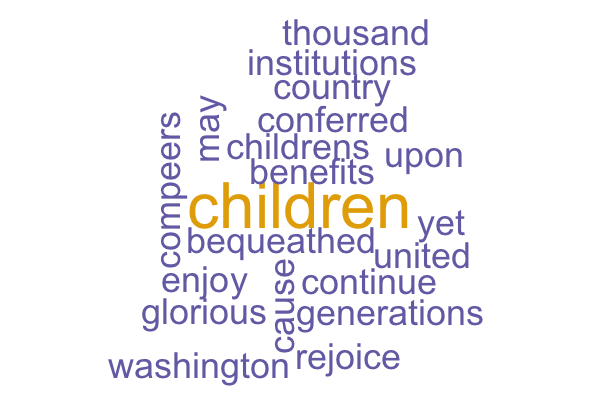
\includegraphics[width=0.3\linewidth]{q1e1.png}
		\caption{Question 1 Part 1}
	\end{figure}
	
	\item \textbf{Inclusions} = ['thousand',  'institutions', 'enjoy', 'conferred', 'cause', 'benefits', 'children', 'bequeathed', 'childrens', 'continue', 'generations', 'glorious', 'united', 'yet', 'may', 'country', 'upon', 'rejoice', 'Washington', 'compeers'] .
	\\
	\textbf{Exclusions} = ['under', 'his', 'us', 'to', 'those', 'and', 'our', 'the', 'a', 'have', 'by']\\
	\\
	Wordcloud removes stopwords which is why some words are included and others are excluded. This is because we passed a string and left the frequency parameter unspecified which results in stopword removal.
	
	\item \textbf{Sentence}: "Operational Incident affecting application hosted on MuleSoft Anypoint Platform occurs.
	Organization operational support resources perform necessary initial incident assessment and triage.
	Decision: is assistance required from MuleSoft support to assist with incident diagnosis or resolution?
	Gather the minimum information required based on the profile of the incident. Please see: section below for minimum information that is required when opening a support a ticket." 
	\\
	\textbf{Plot}:
	\begin{figure}[h!]
		\centering
		
\includegraphics[width=0.3\linewidth]{q1e2.png}
		\caption{Question 1 Part 3}
	\end{figure}
	\\
	\textbf{Inclusions}: Required, Incident, Support
	\\ 
	\textbf{Exclusions}: All words are excluded except the three above.
	\\
	While my hypothesis that stopwords are excluded is validated, we see that fewer words are returned than we would expect if only stopwords were removed. Checking the wordcloud documentation \href{https://www.rdocumentation.org/packages/wordcloud/versions/2.6/topics/wordcloud}{here} we see that while stopwords are removed if the text is passed as a string and frequency is not set, we can also see a default minimum frequency of three is set (it's not clear to me why this is not impacted in the first part of this question).\\
	
	\item Repeating some words multiple times with the new sentence:
	\\
	"Operational Operational Operational Incident affecting affecting affecting application hosted on MuleSoft Anypoint Platform occurs.
	Organization operational support support resources perform perform perform perform necessary necessary necessary initial incident assessment and triage.
	Decision: is assistance required from MuleSoft  MuleSoft MuleSoft MuleSoft MuleSoft MuleSoft support to assist with incident diagnosis or resolution?
	Gather the minimum information required based on the profile of the incident. Please see: section below for minimum information that is required when opening a support a ticket."
	\\
	\textbf{Plot}:
	\begin{figure}[!h]
		\centering
		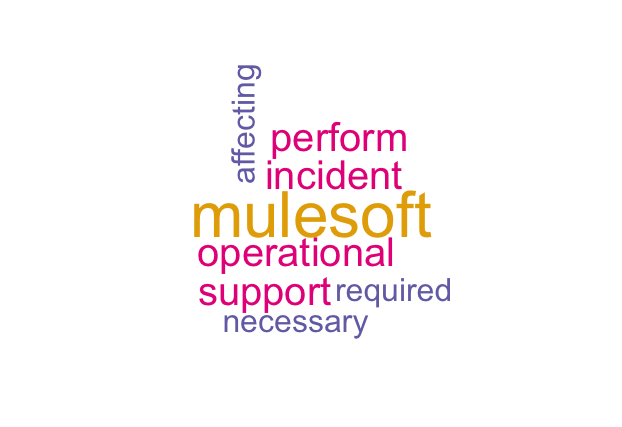
\includegraphics[width=0.3\linewidth]{q1e3.png}
		\caption{Question 1 Part 4}
	\end{figure}
	\\
	We see our repeated words that appear three or more times are now included. While it's still not clear to me as to why words which appeared less than three times appear in the wordcloud in the original text provided, we see by passing in the parameter min.freq=1 that we can alter this behaviour to produce the below:
		\begin{figure}[!h]
		\centering
		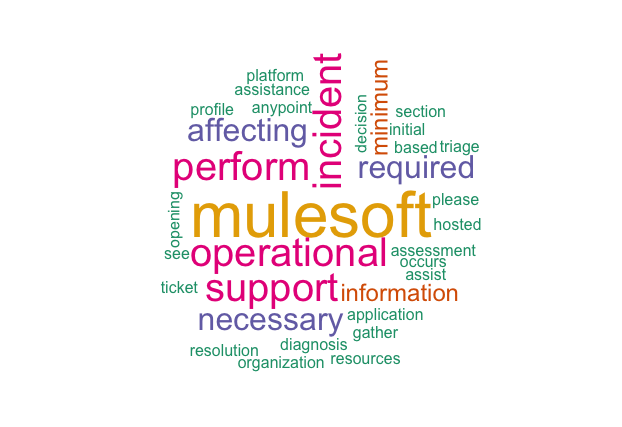
\includegraphics[width=0.3\linewidth]{q1e4.png}
		\caption{Question 1 Part 4 ii}
	\end{figure}
	
	
	
\end{enumerate}

	

\section{Exercise 2}
This is the answer to question 2.
\begin{enumerate}
	\item The key peaks we see are approximately in 1820, 1955, 1970, 1975, and 2001. For the 19th century peak, we see "Mark Keane" is featured in "Reports from Committees" for the British House of Commons in this time period. In the 1954-1956, we see Mark Keane (\href{https://www.legacy.com/us/obituaries/chicagotribune/name/mark-keane-obituary?id=2652673}{here}) was the name of a village manager in Oak Park Illinois resulting in this appearing in public service bulletins. By the 1970s peak we see Mark Keane was an executive director of the International City Management Association resulting in a greater volume of publications referring to him through government documents. The 2001 peak primarily stems from UCD lecturer Mark Keane's publications in psychology, cognitive science, and computer science.
	\item Adam Ryan has peaks in 1812, the 1940s, and 2008-2010. The hits in 1812 are predominantly driven by false hits from co-authors with a first name of Adam and a first name (or surname) of Ryan but not a single individual. A putting quotes around the name in this time period reveals no hits. In the 1940s Adam Ryan peaks due to a publication in the Proceedings of the National Tax Association however, again, this is an incorrect citation from one attendant named "Adam Rumoshovsky" and "Frank J Ryan" which, due to their formatting, is captured as "Adam Ryan" in NGram. An Adam Ryan from Philadelphia set a Ring Record resulting in his publication in "Nat Fleischer's All-time Ring Record Book" in 1943. The peak in 2008-2010 does not stem from a singular Adam Ryan, but is present due to an increasing usage of the name both in fiction, a Benedictine monk named Adam Ryan resulting in publications in religious texts, and in society at large resulting in references to numerous students/children/workers called Adam Ryan.
	\item The word I chose is "Tweet" which is used to refer in its modern form to the act of posting on Twitter. We see that, in fact, it is actually a relatively recent word in its usage. While The earliest usages of it pre-Twitter stem from onomatopoeic references to birds, or characters named tweet, it's explosion in usage coincides with the introduction of social media and the altering of meaning of the word.
	\begin{figure}[!h]
		\centering
		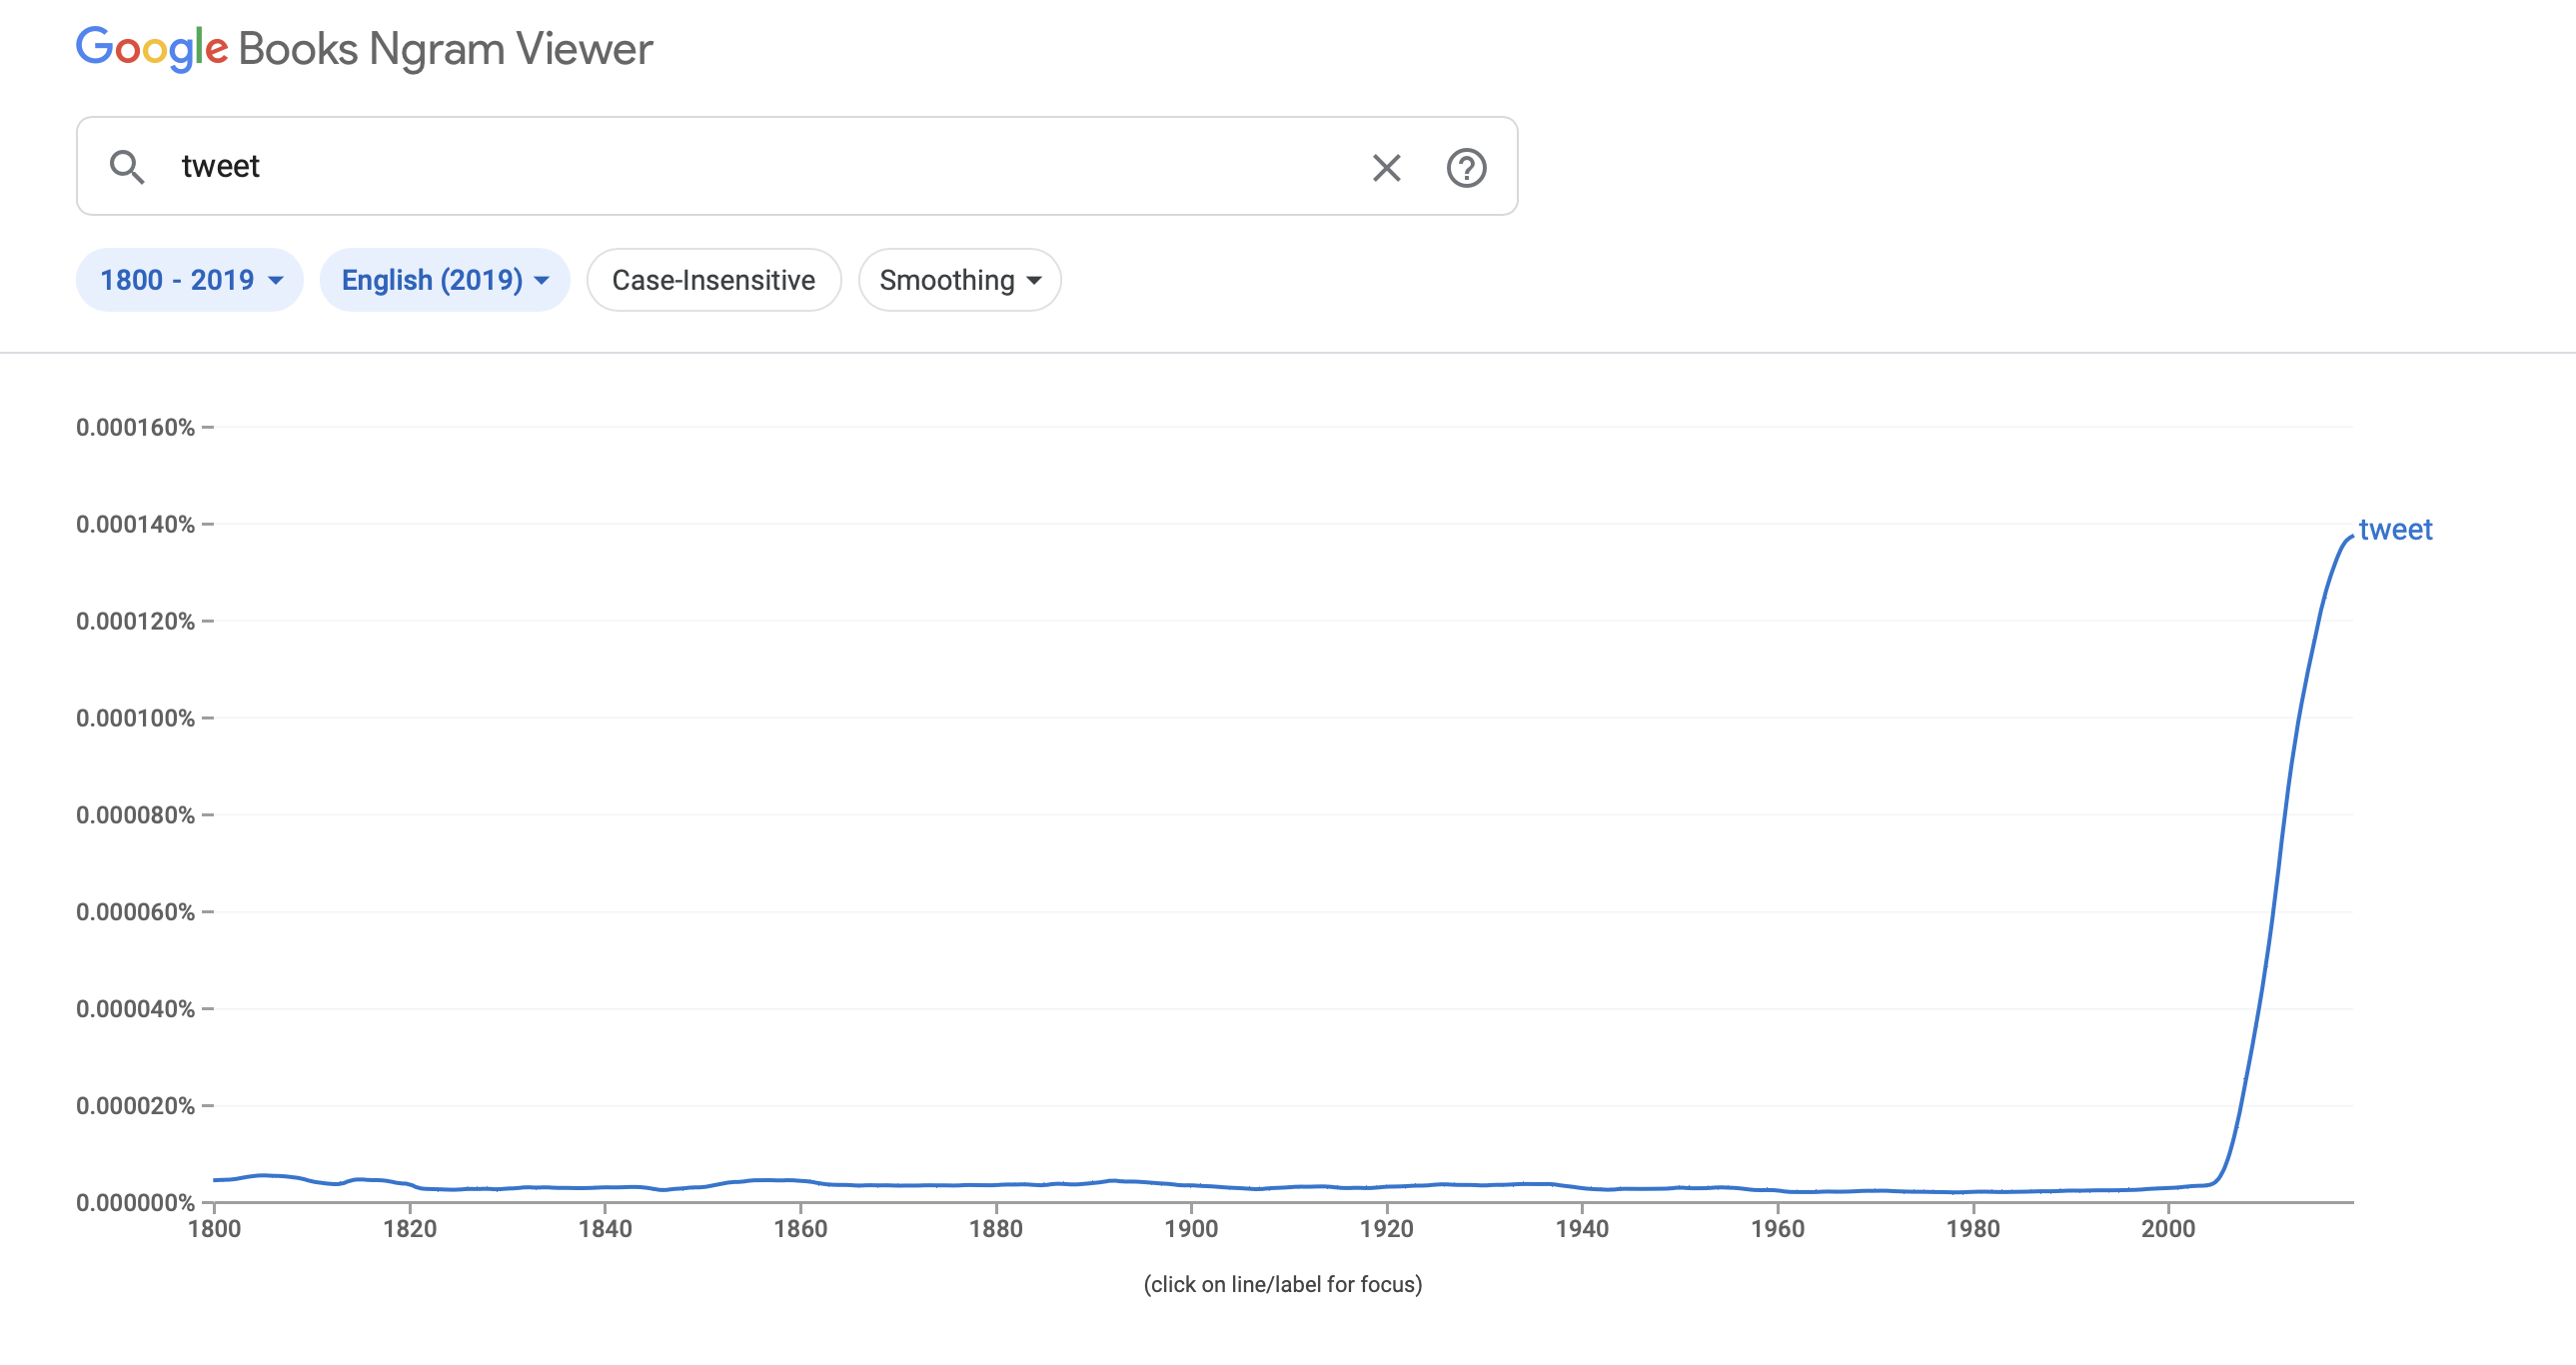
\includegraphics[width=0.3\linewidth]{q2e3.png}
		\caption{Question 2 Part 3}
	\end{figure}

\item I've looked at the term "Reusable Energy" as the other graphs were relatively uninteresting with smoothing. The results of various smoothing is shown n figures \ref{NoSmooth}, \ref{ThreeSmooth}, \ref{SixSmooth}.  Smoothing these searches smoothes some of the blips which occur in the charts by averaging values over the number of years chosen (\href{https://port.sas.ac.uk/mod/book/view.php?id=554&chapterid=328}{per here})to make it easier to analyse the trend over time. Smoothing reusable energy over three years, we more easily see the peaks, while over six years we see it was a prominent term in literature from 1960 to 2000

\begin{figure}[h!]
	\centering
	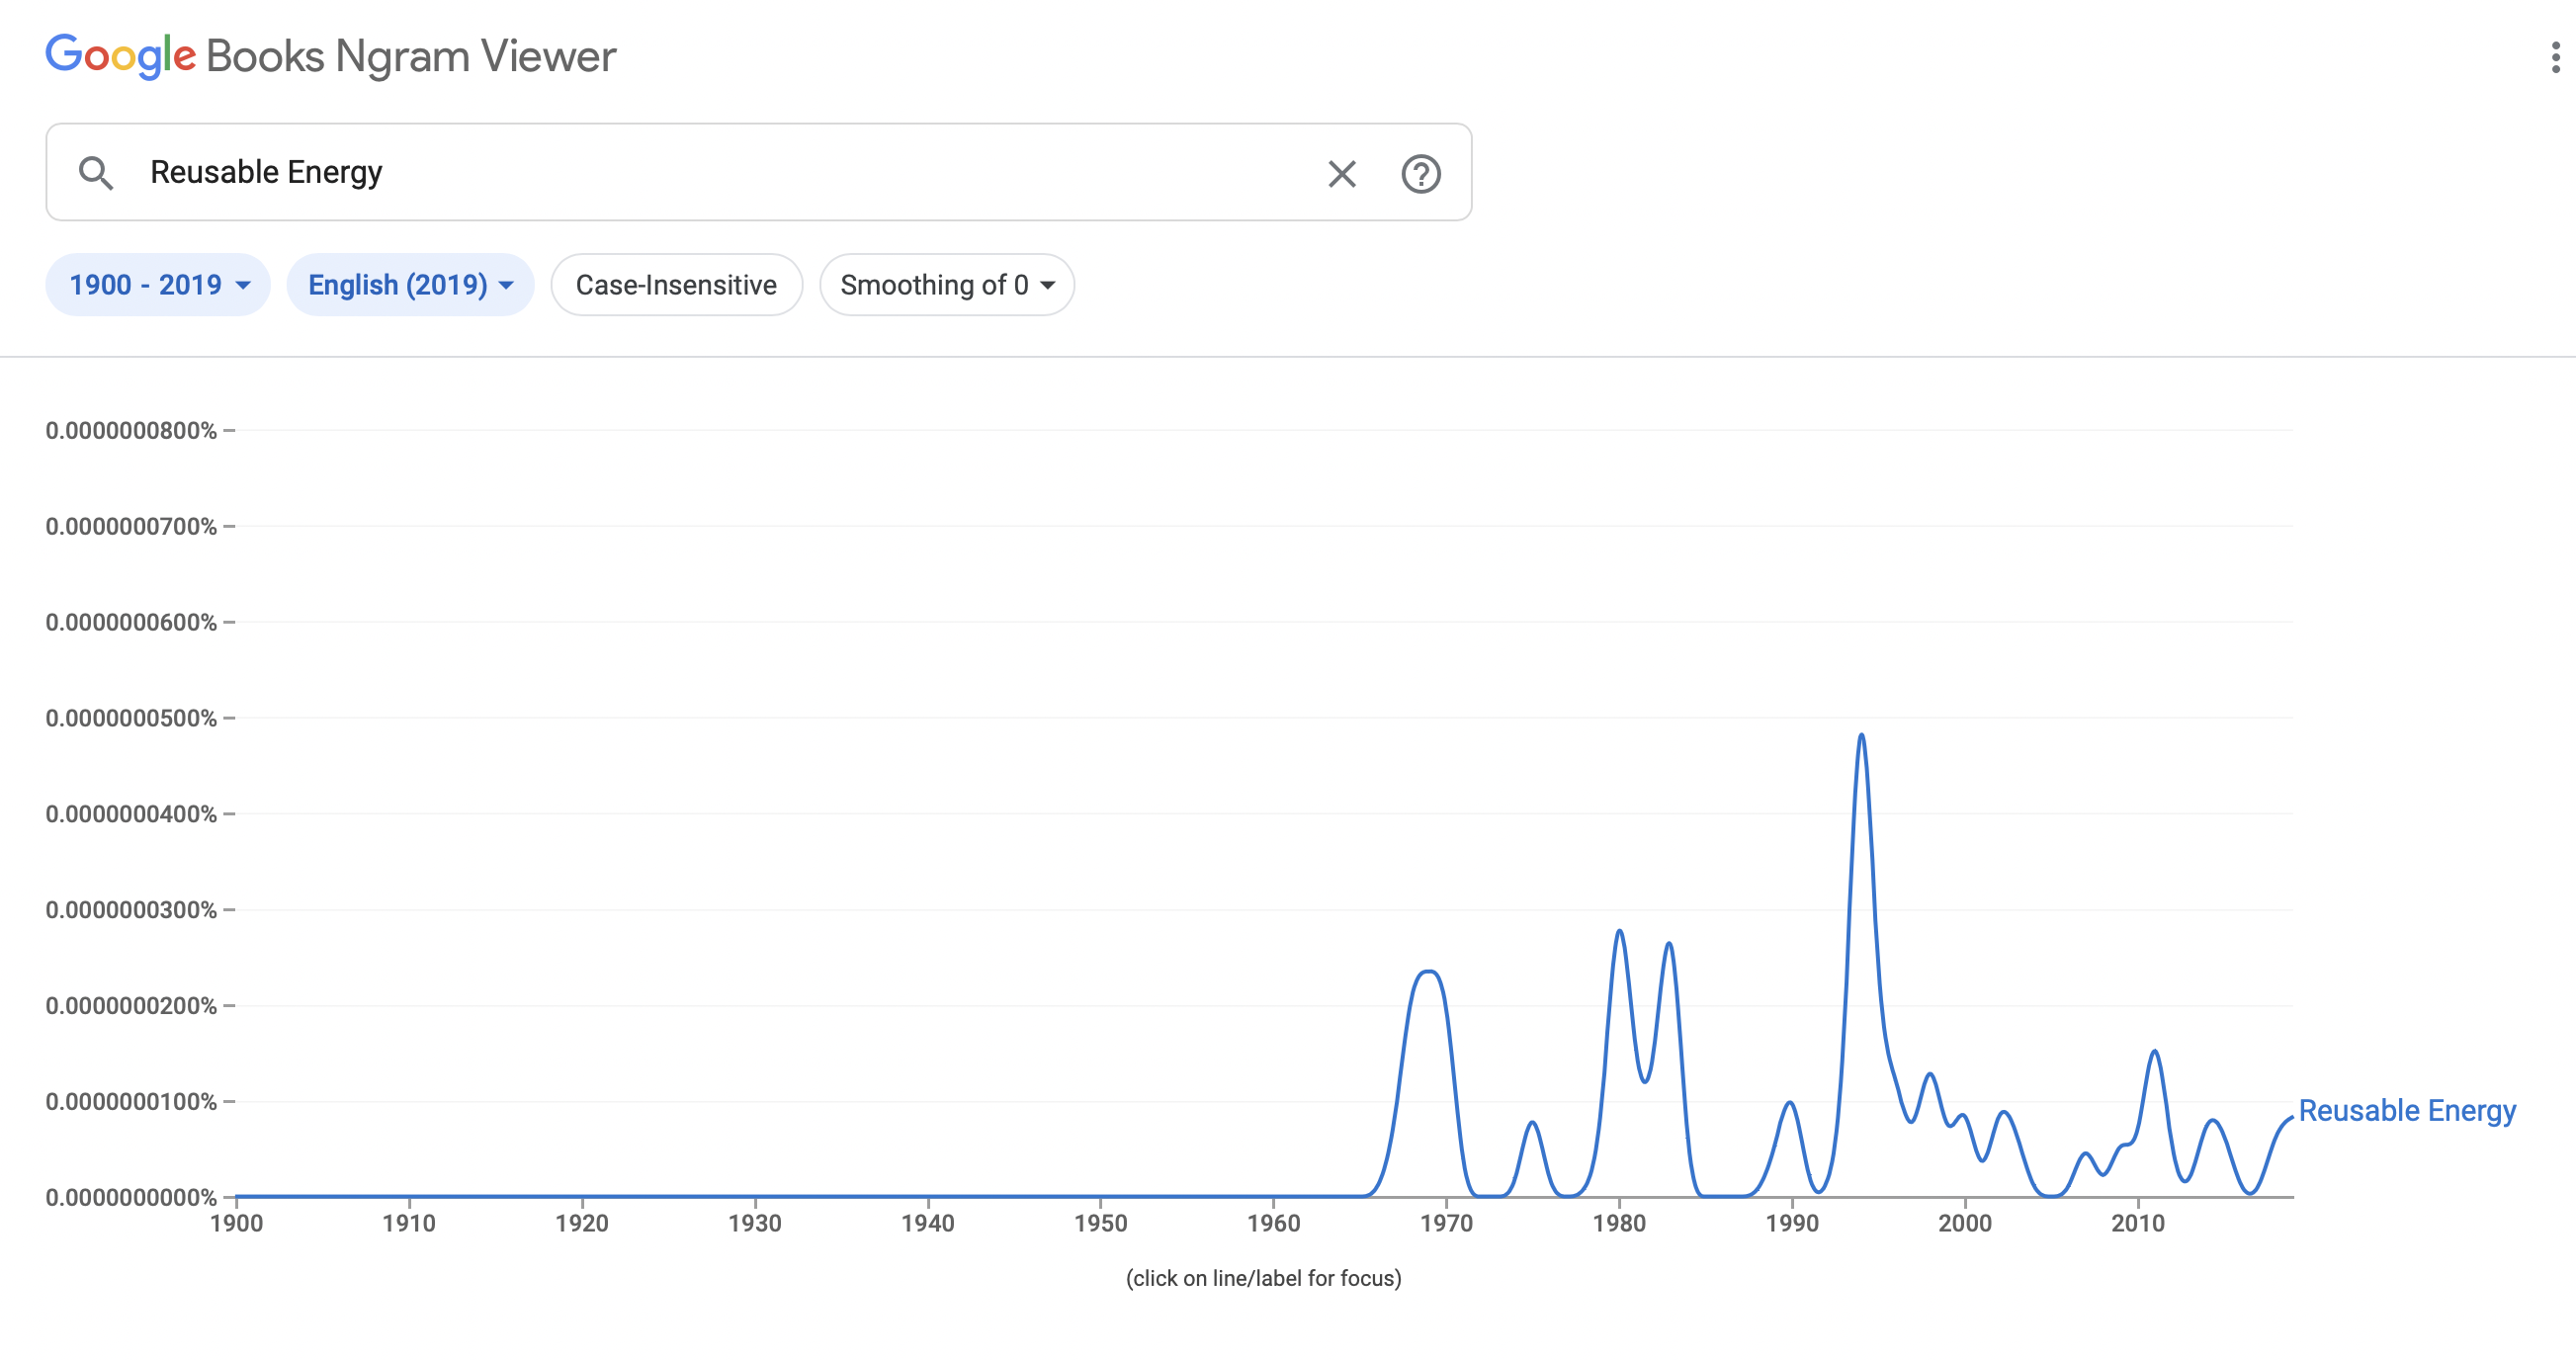
\includegraphics[width=0.4\linewidth]{re_sm0.png}
	\caption{Q2P4 Smoothing=0}\label{NoSmooth}
\end{figure}
\begin{figure}[h!]
	\centering
	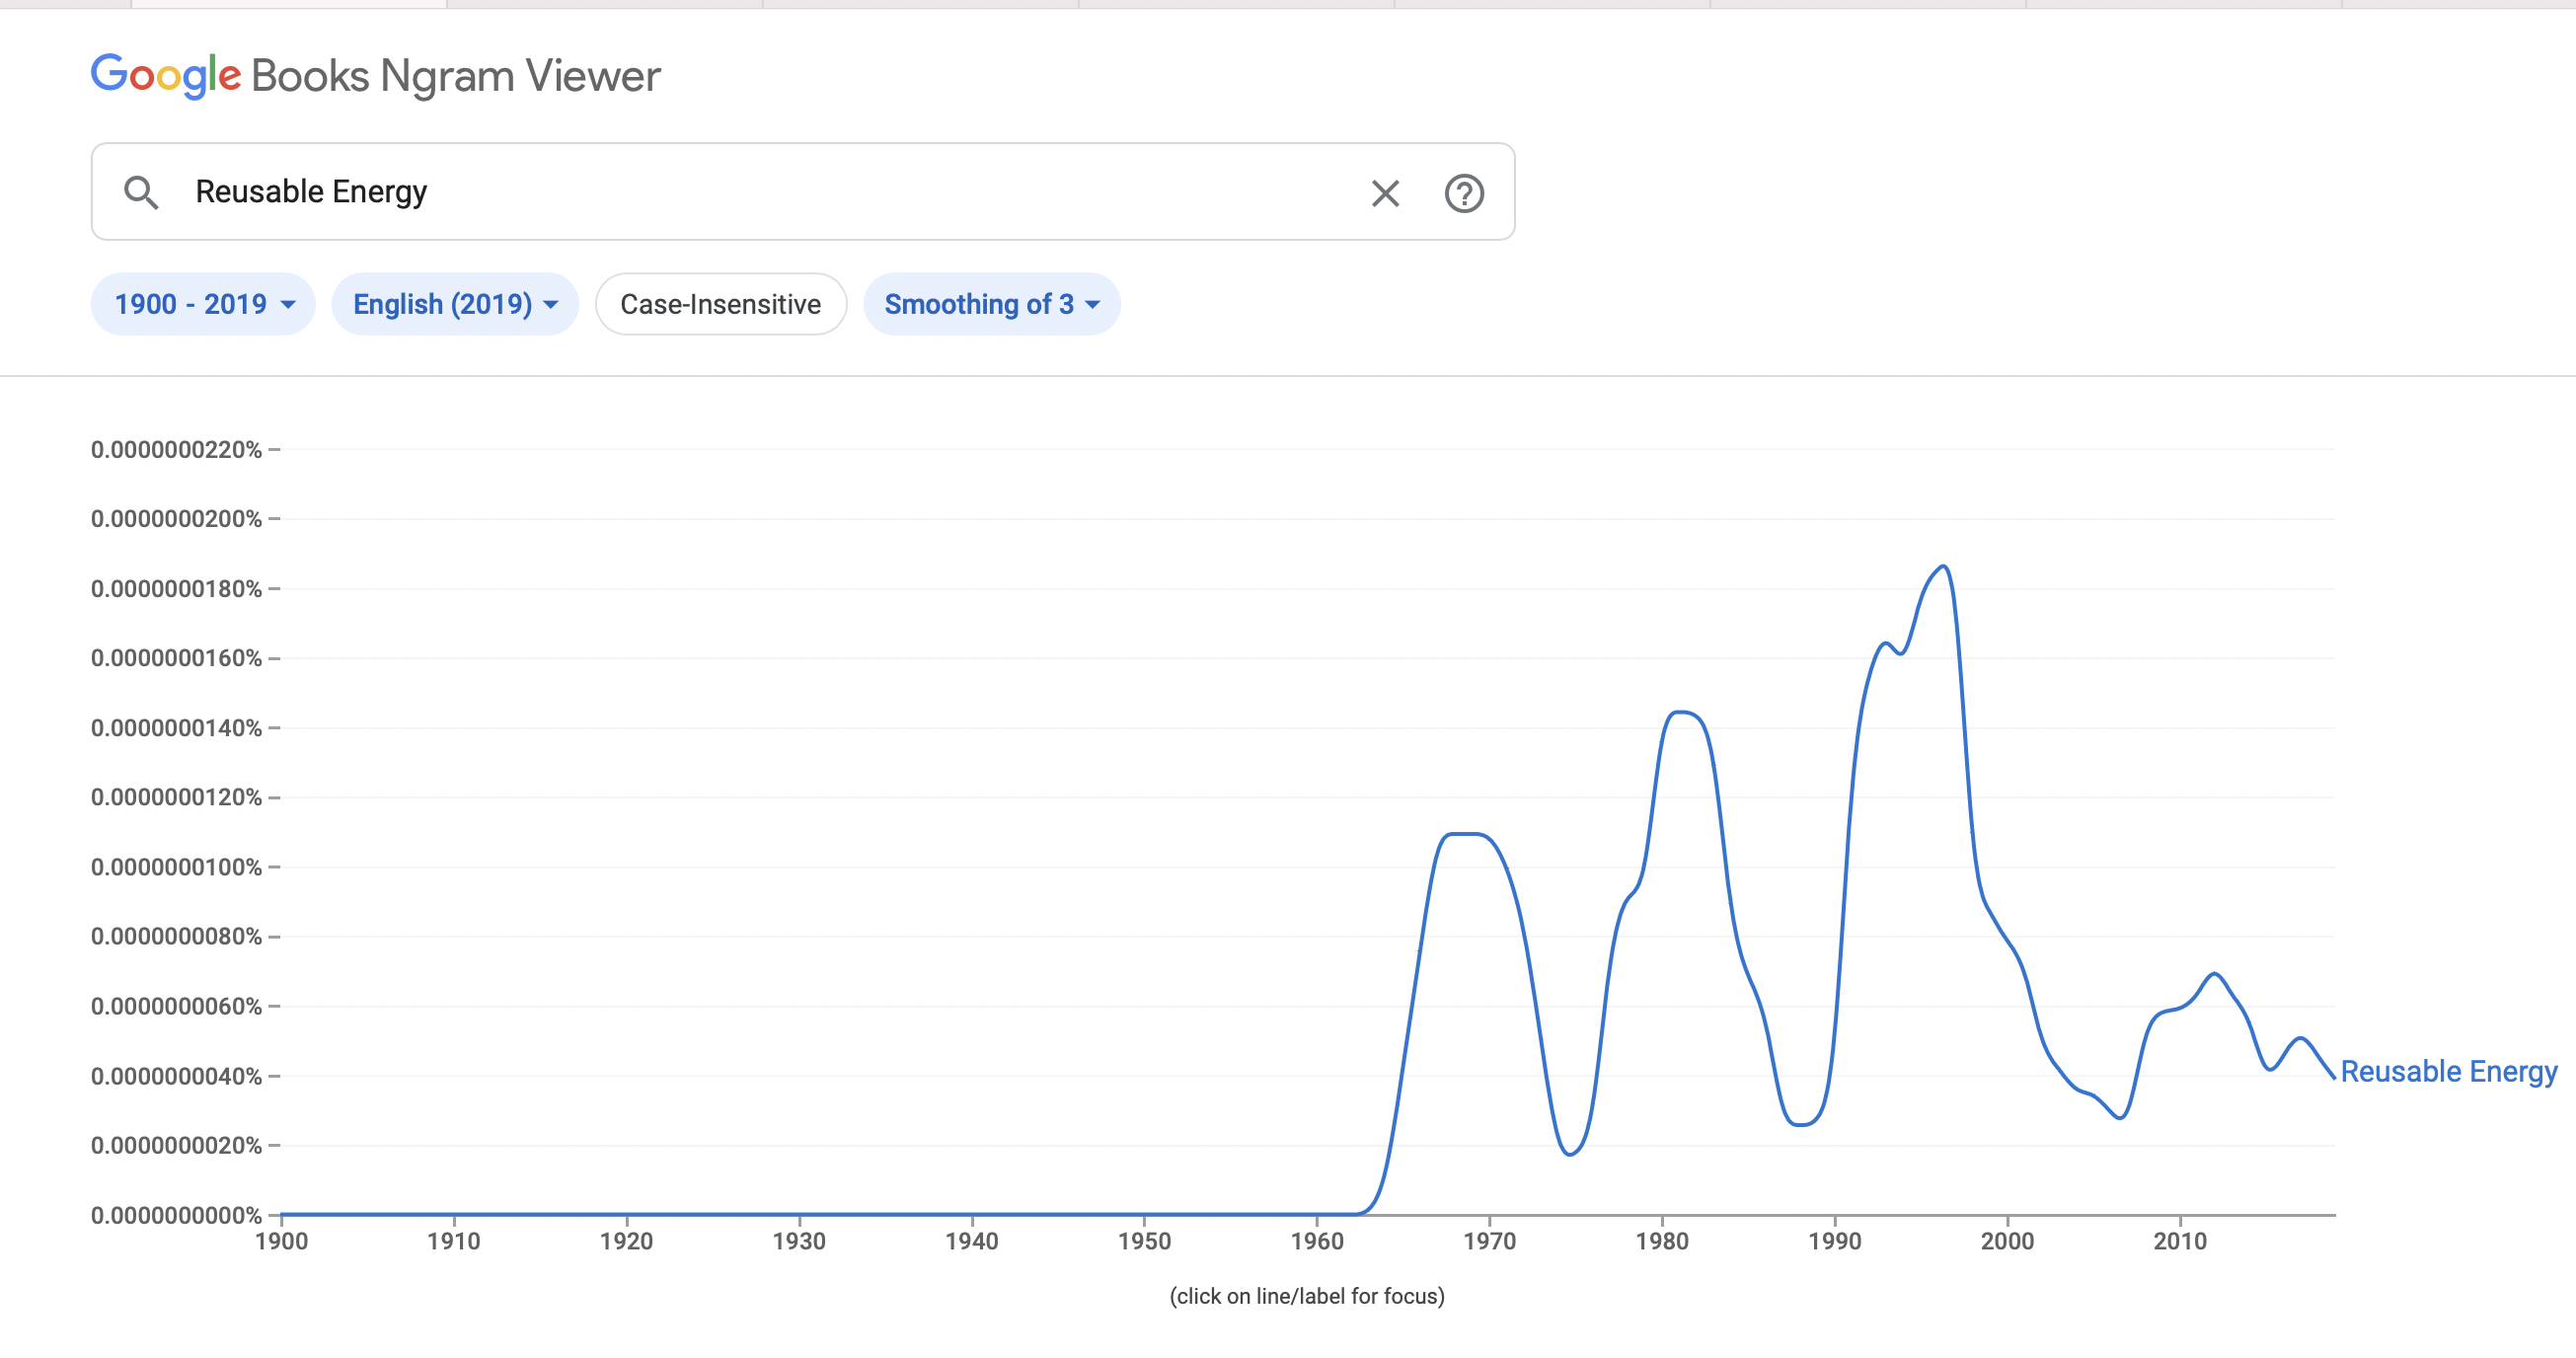
\includegraphics[width=0.4\linewidth]{re_sm3.png}
	\caption{Q2P4 Smoothing=3}\label{ThreeSmooth}
\end{figure}
\begin{figure}[h!]
	\centering
	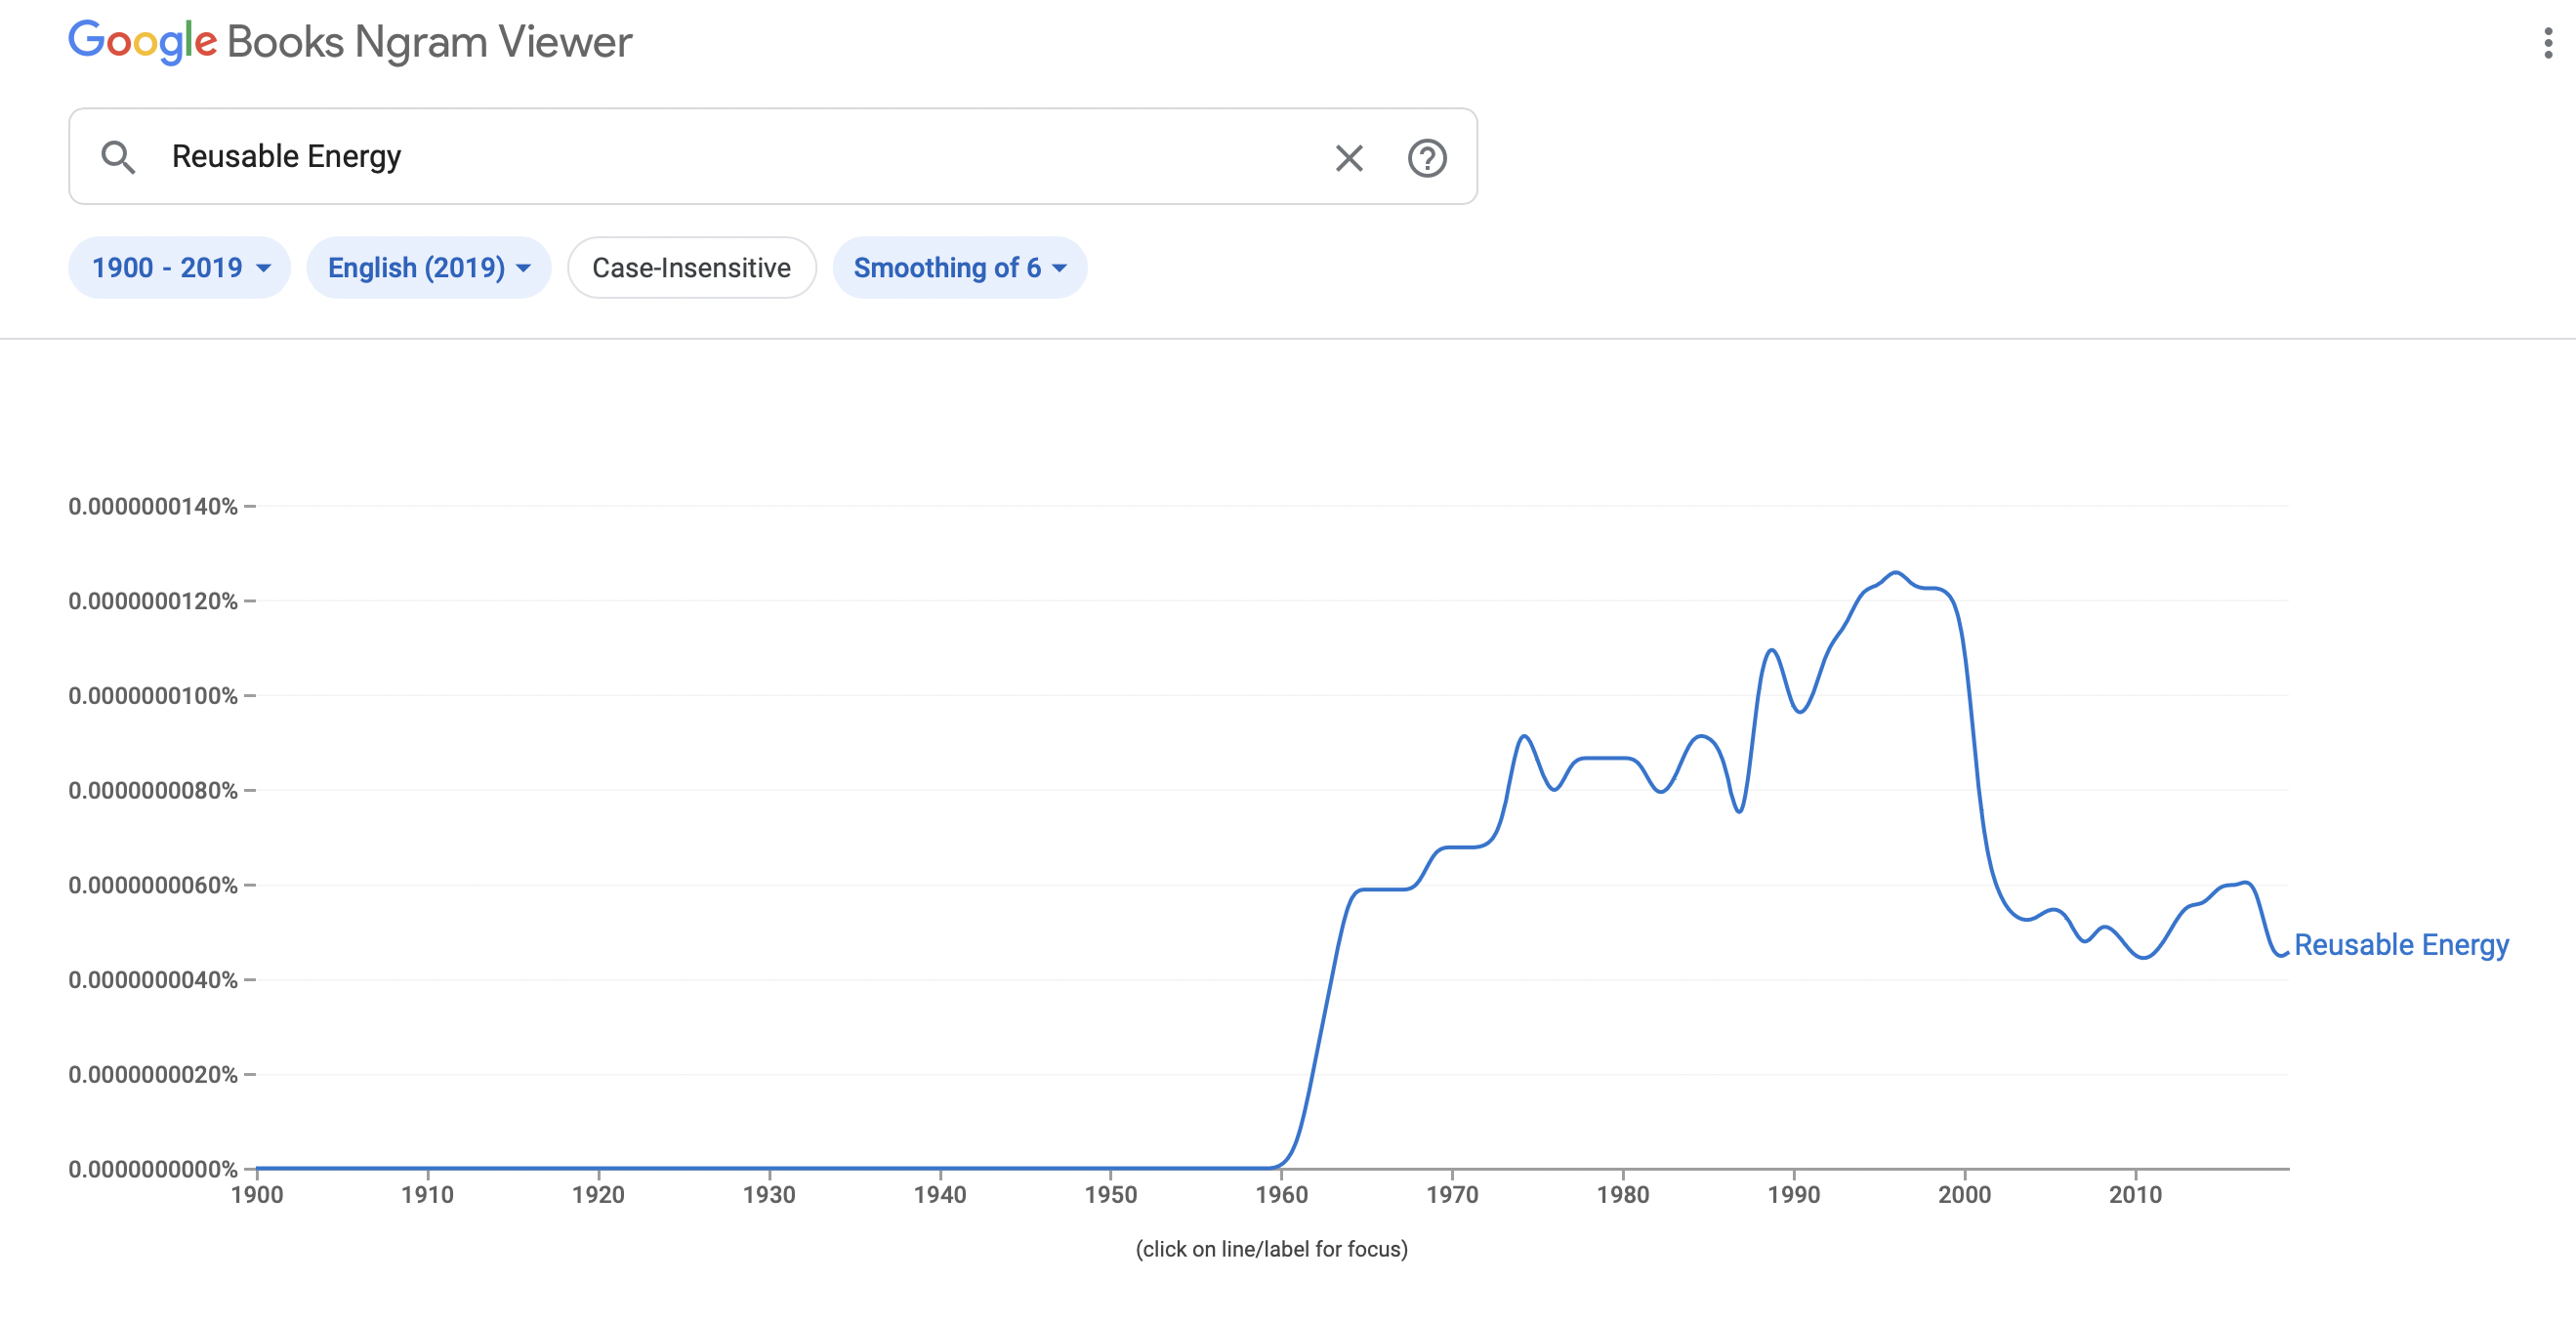
\includegraphics[width=0.4\linewidth]{re_sm6.png}
	\caption{Q2P4 Smoothing=6}\label{SixSmooth}
\end{figure}
\item The terms I chose to plot were "Lannister, Greyjoy, Targaryen, Baratheon, Westeros". Each of these terms are surnames, with the exception of Westeros which is the setting,  in the series "A Song of Ice and Fire" which was first published in 1996 and brought to prominence by the TV series in 2011. By observing figure \ref{GOT} we see that prior to the television show, the 'Lannister' characters are the most referenced from publication to air date due to the high volume of 'Lannister' characters. Following airing, we see during the initial year of publication, this term significantly rose in prominence while the other surnames experienced an influx in prevalence. Interestingly we see dips in each term between seasons, and as the relevance of certian characters on the plot became increasingly prominent (Targaryen) and as the world of the show expanded via other novels ("The World of Ice and Fire") references to these characters increased in prominence while references to Lannisters (previously highly central characters but less prominent as the show progressed) fell to become less prominent than references to the show's overall universe of Westeros. What is particularly interesting to me is how the references to the surnames split in 2012 after previously being relatively equal (with the exception of the Lannisters)
\begin{figure}[h!]
	\centering
	\includegraphics[width=0.6\linewidth]{got.png}
	\caption{Game of Thrones Characters}\label{GOT}
\end{figure}
\item To use POS tags \href{https://books.google.com/ngrams/info}{here} for details. I plot the noun 'Tweet' against the verb 'Tweet'. We see that the noun 'tweet', referring to messages on the socia media platform Twitter or the noise of a bird, outpaced the growth of references to the action of tweeting (to post on the platform, or, for a bird, to chirp) as the platform grew, with the rate of growth of the noun rising faster than the verb which flattened around 2014.
\begin{figure}[h!]
	\centering
	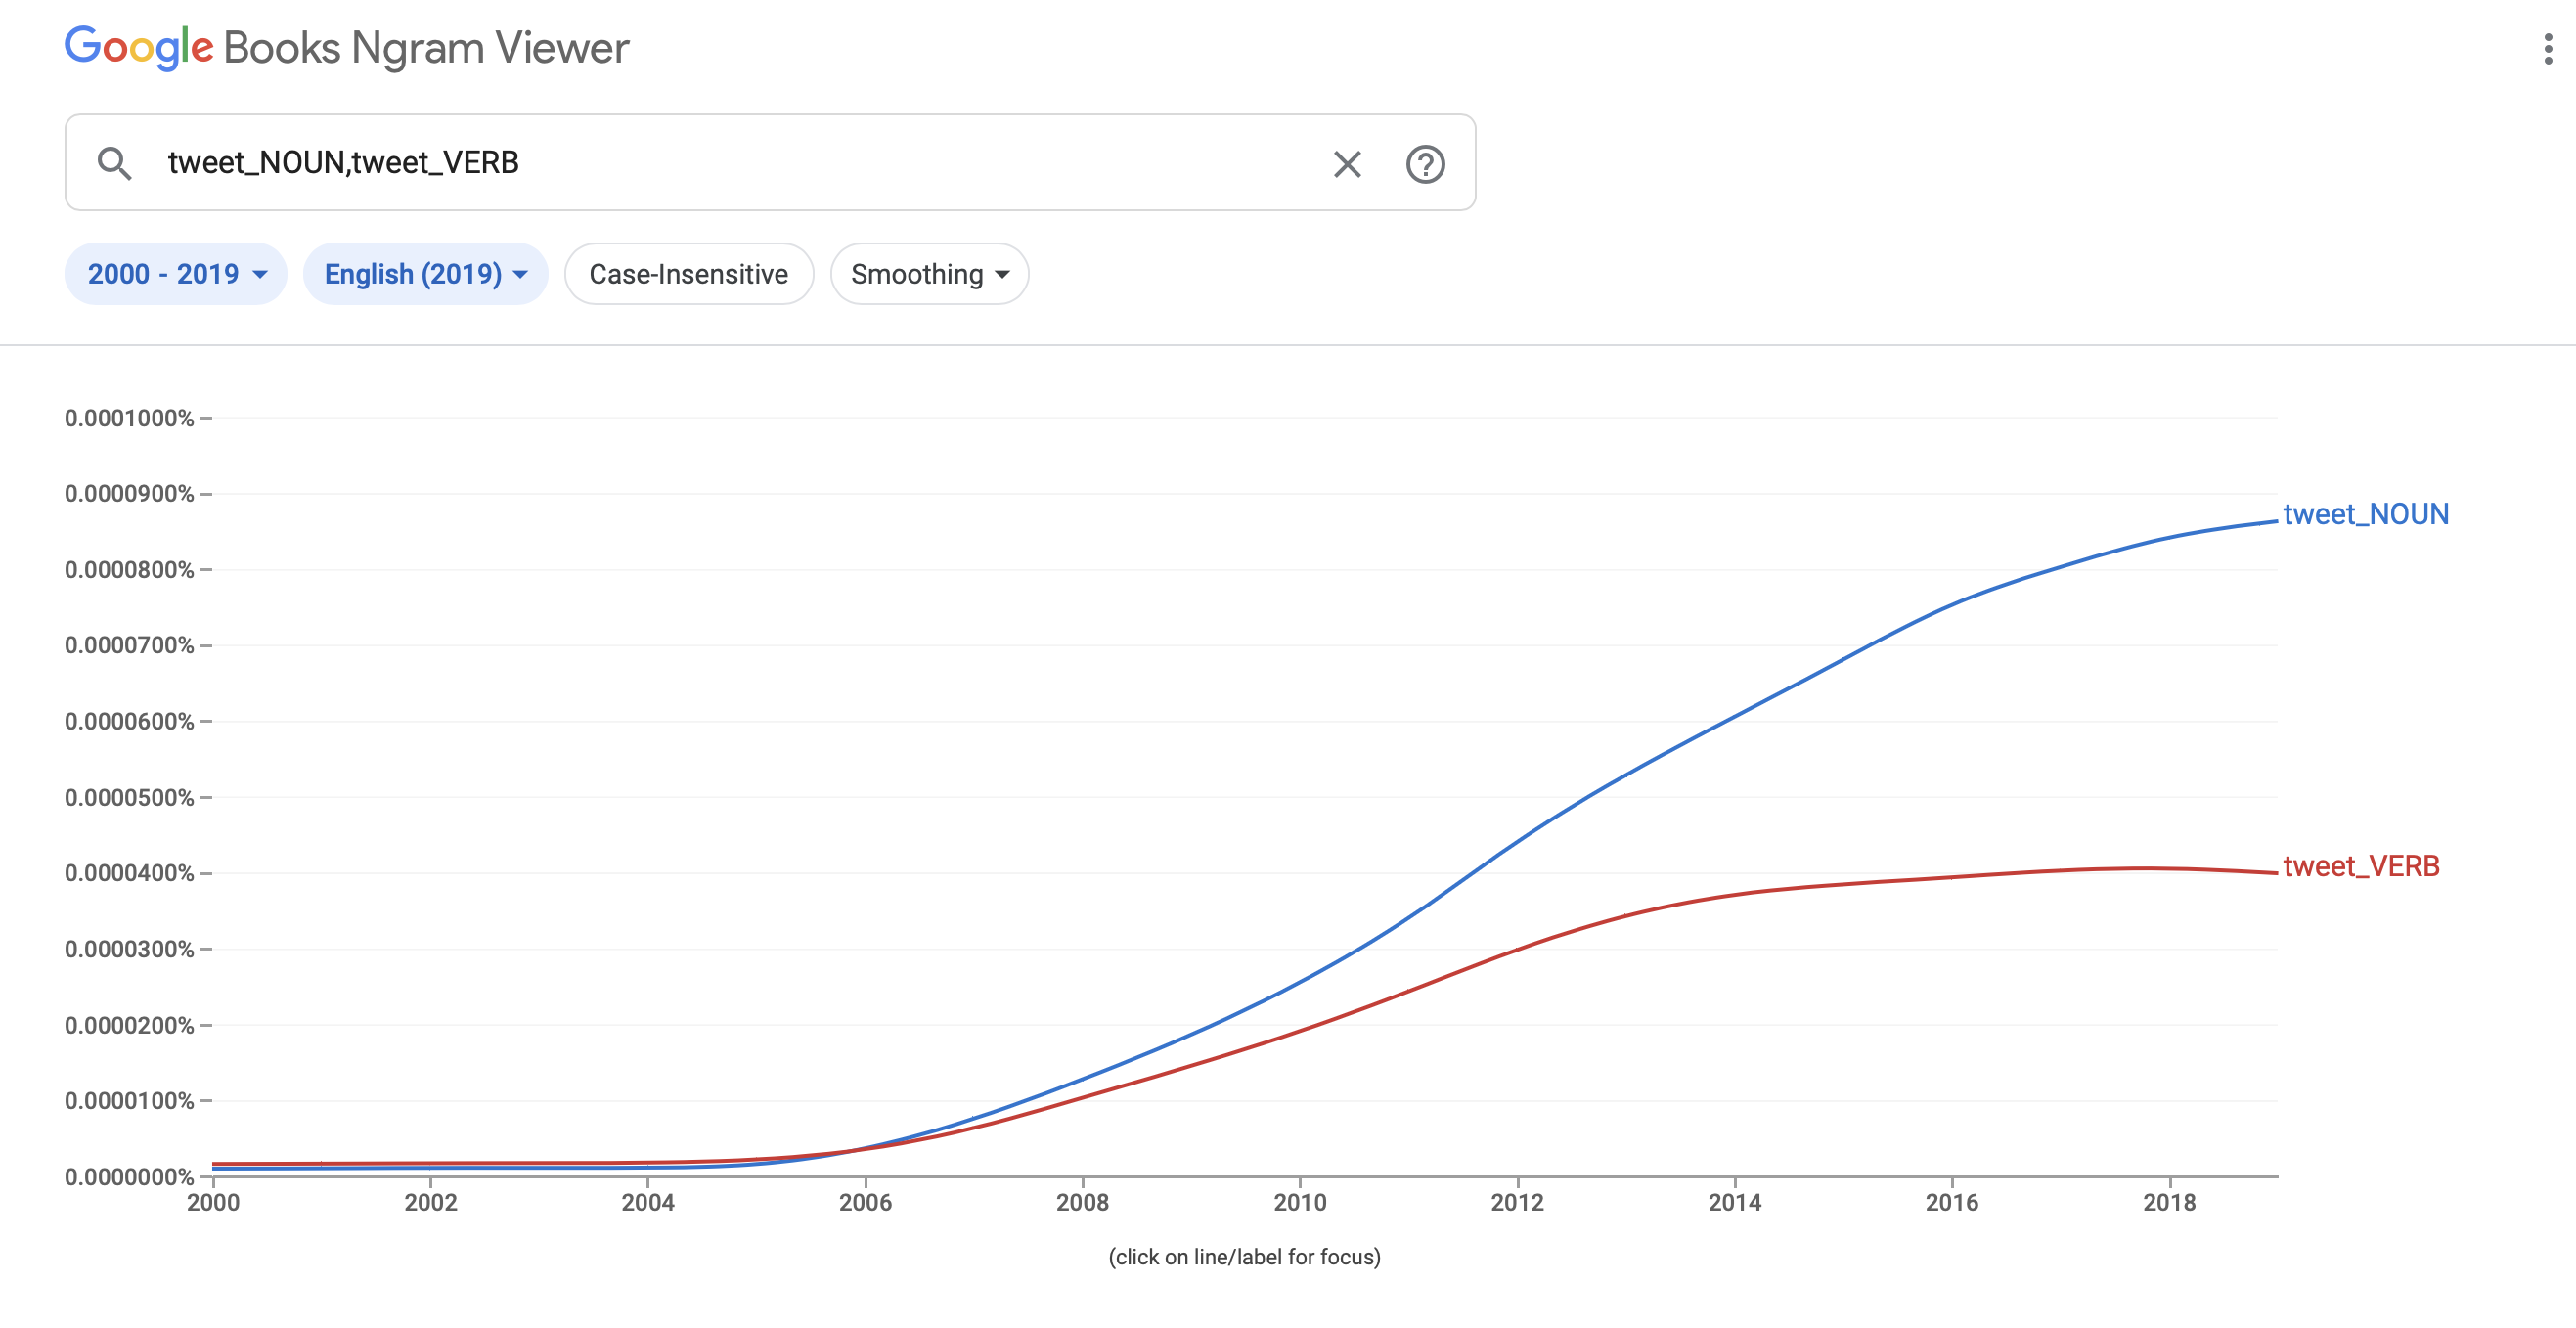
\includegraphics[width=0.5\linewidth]{tweet.png}
	\caption{Tweet\_Noun vs Tweet\_Verb}\label{Tweet}
\end{figure}
\item One of the key events which happened over the last 500 years is the Cold War which emerged at the end of the second world war, and a key cultural effect this had was in the creation of terror surrounding communism and socialism in the United States. We see through Google NGram that references to socialist and communist dramatically increase following the end of the second world war, and decline following the end of the Cold War, while references to 'nuclear' similarly spike at a time when the fear of nuclear war between the Soviet Union and US was a pervasive cultural fear; this term in particular reaches its apex with the Chernobyl disaster in the mid-1980s, however, we can clearly see this had spiked during the height of the Cold War. The Space Race was a key component of the Cold War, and we see references to space peak during this time (unsurprisingly with the Moon Landing). Finally, following the fall of the Soviet Union, we see a dramatic decrease in the usage of the word soviet. The key cultural impact of this event (the Cold War) was the impact on the villification of communism and socialism in the United States, combined with the impact this had on fear of nuclear war, and both of these aspects can be clearly seen by their relative emergence towards the end of the second World War, and the subsequent pronounced spikes during the middle of the Cold War.
\begin{figure}[h!]
	\centering
	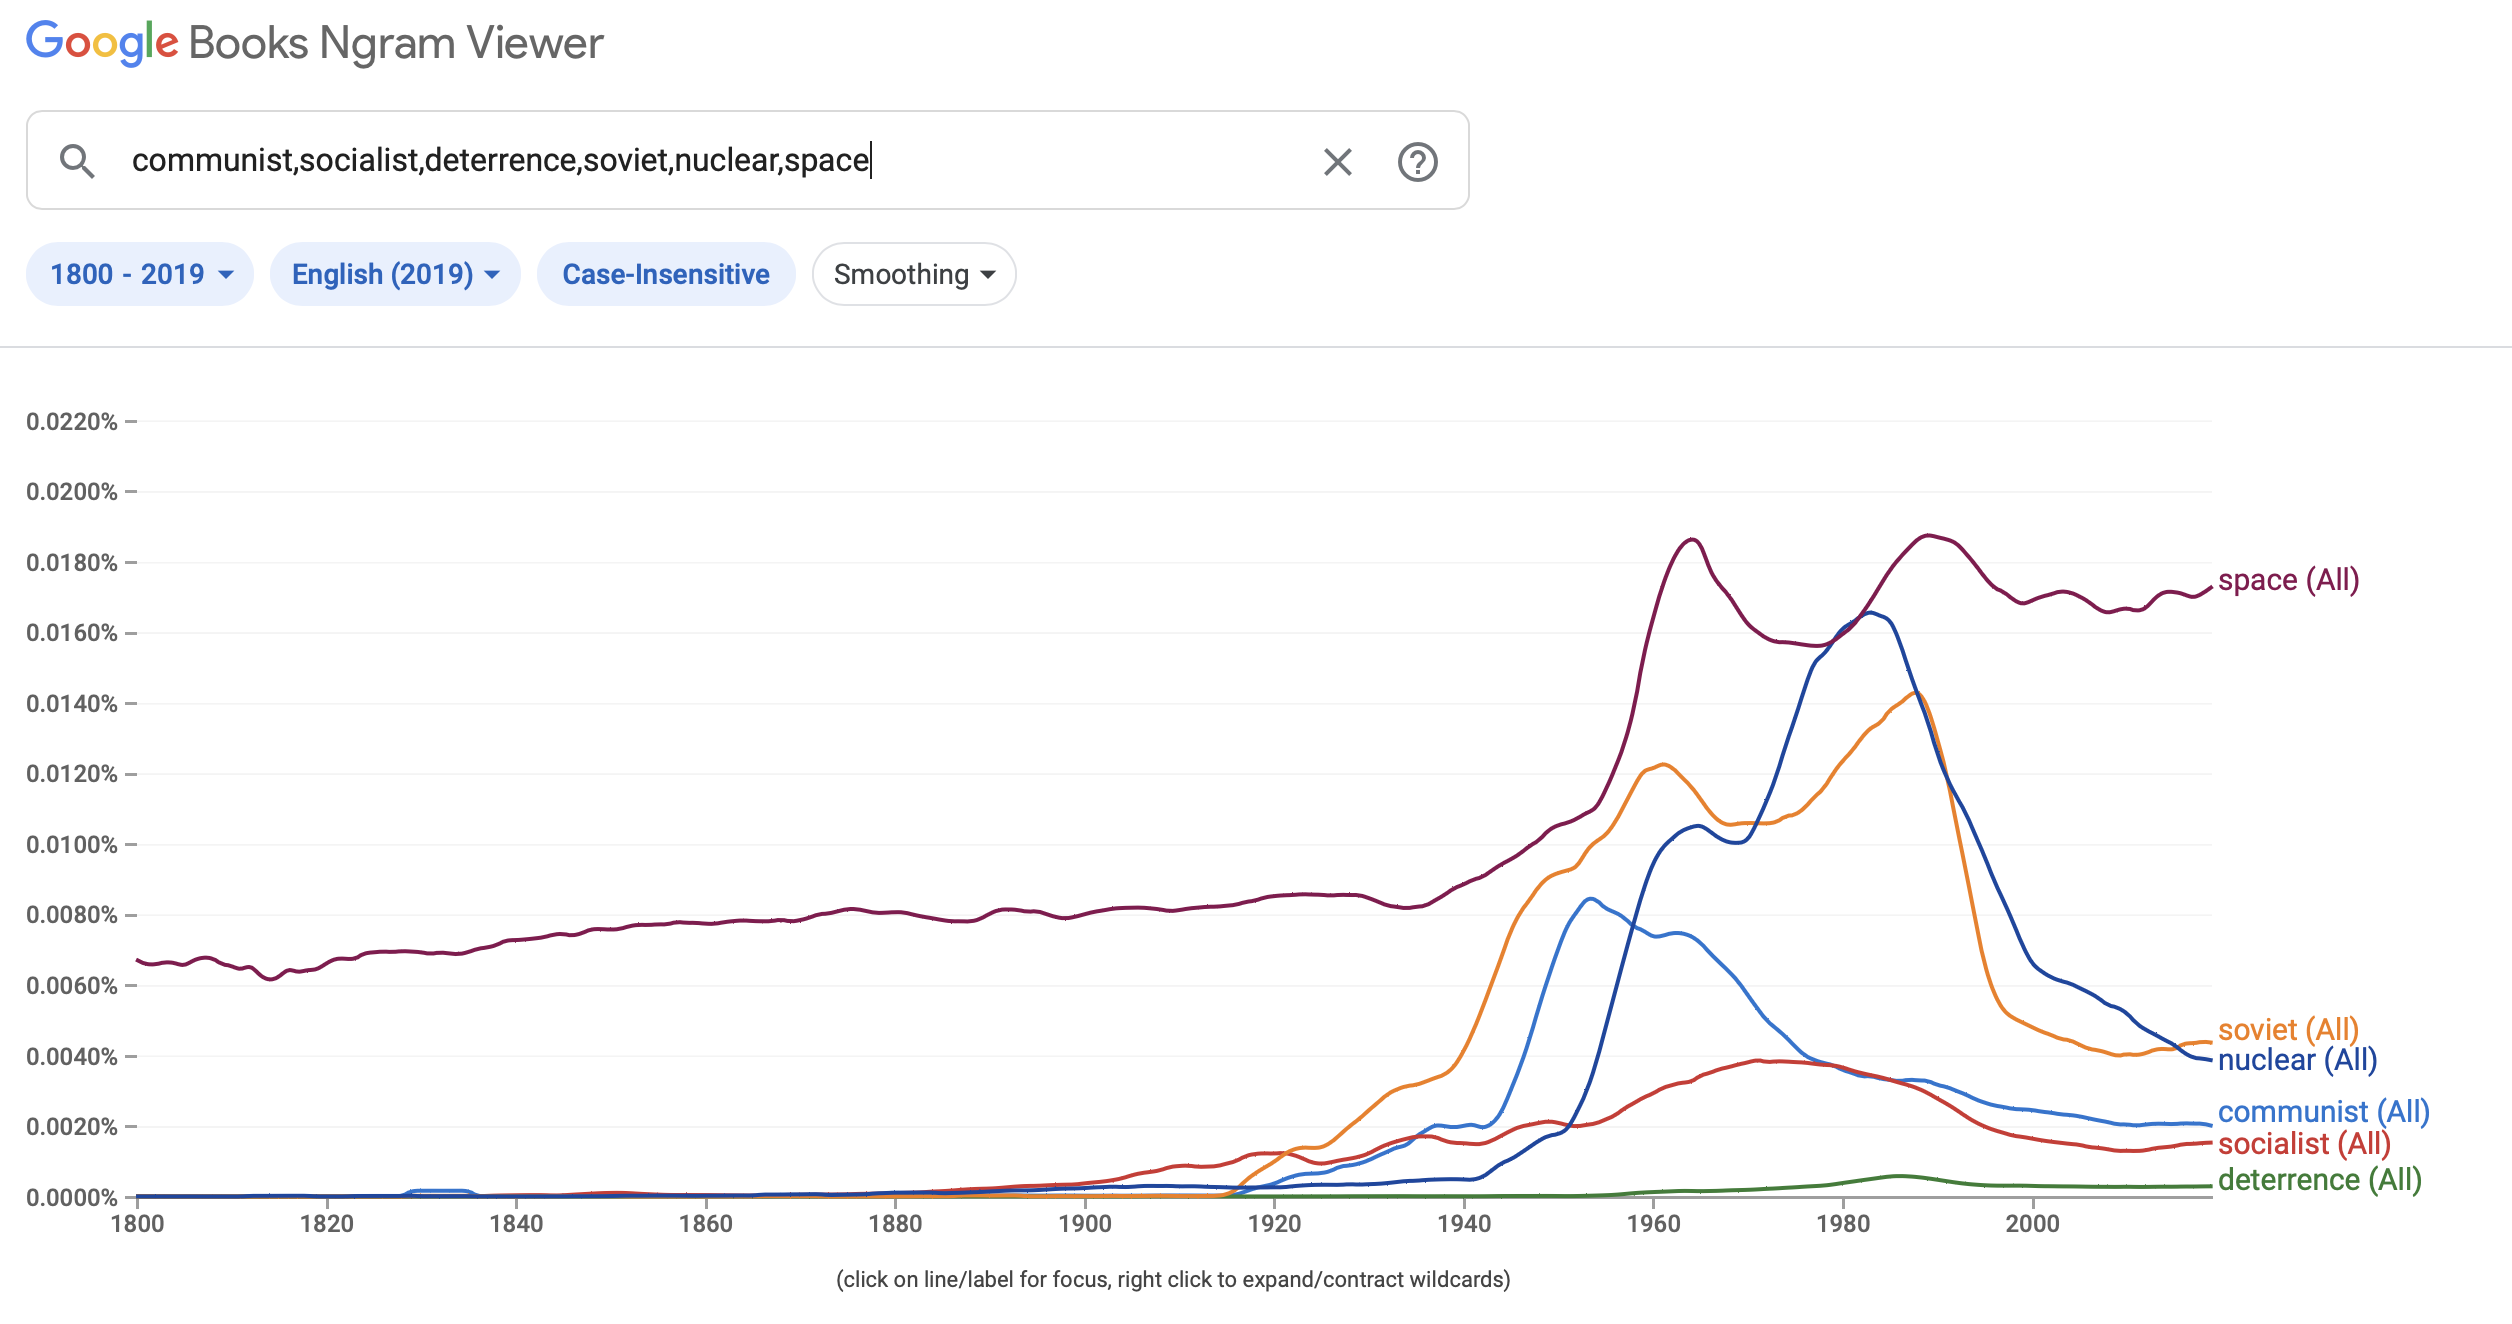
\includegraphics[width=0.4\linewidth]{cold war.png}
	\caption{Cold War references}\label{media}
\end{figure}
\end{enumerate}

	

\section{Exercise 3}
I generate a dataset using the RANDBETWEEN function in Excel and applying this to each of the 15 words across all years. I then normalise. The resulting table is given in figure \ref{q3}
\begin{figure}[h!]
	\centering
	\includegraphics[width=0.95\linewidth]{q3table.png}
	\caption{Raw Data And Normalised Data}\label{q3}
\end{figure}
\begin{enumerate}
	\item For ByYear Normalisation I divide each entry in the year by the total words in that year (see formula in table). I set these to a percentage for legibility.
	\item For Overall Normalisation, I divide each entry in the year by the total sum of words (all raw data entries). I set these to a percentage for legibility.
	\item We see in \ref{table} that there are pronounced differences in the figures obtained. Looking at yearly data, and in observing the change by year, By Year Normalisation is a better view of the frequency on a per-year basis if you are interested in examining individual years and comparing year vs year. If you're interested instead in the dataset as a whole time period (2010 to 2014) rather than specific year-by-year relative change (i.e. you're interested in the prevalence of that word, in the year, out of the entire five year time period), using the overall normalisation may be more appropriate.
\end{enumerate}

\begin{figure}[h!]
	\centering
	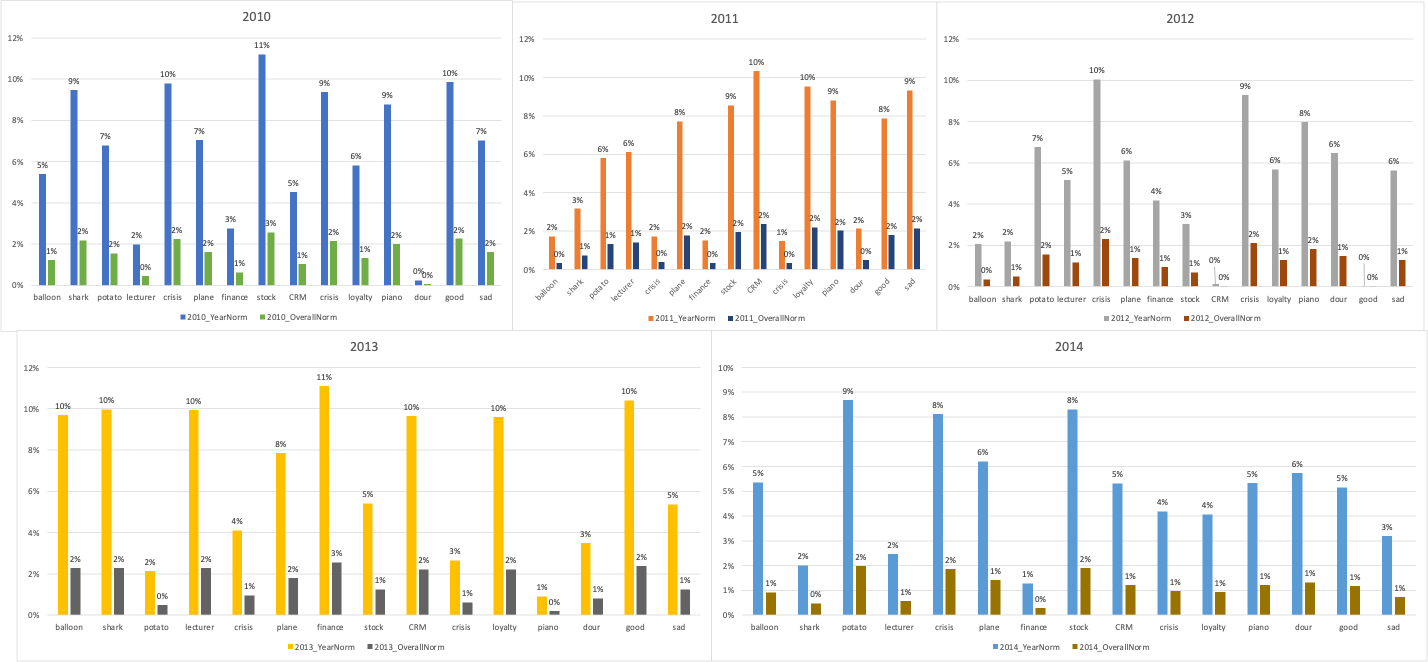
\includegraphics[width=0.95\linewidth]{graphs.png}
	\caption{Normalisation By Year}\label{table}
\end{figure}



	
\end{document}
